\documentclass[12pt,a4paper,titlepage]{article}
\usepackage[utf8]{inputenc}
\usepackage[german]{babel}
\usepackage{amsmath}
\usepackage{amsfonts}
\usepackage{amssymb}
\usepackage{setspace}
\usepackage{graphicx} %Um Bilder anzeigen zu können
\usepackage[top=1in, bottom=1.5in, left=1in, right=1in]{geometry}
\usepackage{endnotes}
\usepackage[section]{placeins}
\usepackage{fancyhdr}
\usepackage{hyperref}

\newcommand{\myma}{\fontfamily{pcr}\selectfont \textbf}
\newcommand{\mymo}{\fontfamily{pcr}\selectfont \textit}
\setlength{\parindent}{0pt}
\let\footnote=\endnote

\begin{document}
\pagestyle{fancy}

\begin{titlepage}
\vspace*{50pt}
\begin{center}
{\Huge Validierung\\[1cm] {\bfseries Praxis der Softwareentwicklung}\\[2cm] Entwicklung einer Software zur Berechnung der Mandatsverteilung im Deutschen Bundestag\\[1cm]Gruppe 1} \\
\vspace*{15pt}
{\normalsize Philipp Löwer, Anton Mehlmann, Manuel Olk, Enes Ördek, \\Simon Schürg, Nick Vlasoff}
\end{center}
\date{}

\vspace*{30pt}
\begin{figure}[h]
\centering
		
\includegraphics[scale=0.6]{KIT-Logo.png}\\
		\vspace*{10pt}
		\Huge WS 2013 / 14
\end{figure}
\end{titlepage}
\newpage\thispagestyle{empty}\hspace{1em}\newpage
\def\Vhrulefill{\leavevmode\leaders\hrule height 0.7ex depth \dimexpr0.4pt-0.7ex\hfill\kern0pt}
\cfoot{{\Vhrulefill~  Seite \thepage   ~\Vhrulefill} \newline {\scriptsize KIT – Universität des Landes Baden-Württemberg und nationales Forschungszentrum in der Helmholtz-Gemeinschaft}}

\pagenumbering{roman} 

 
\newpage
\begin{onehalfspace}
\tableofcontents
\end{onehalfspace}
\newpage

\pagenumbering{arabic} 

\section{Einleitung}

Ziel der Validierungsphase war es das fertige Software-Produkt zu überprüfen um die möglichst fehlerfreie Funktionsweise der Software bestmöglich zu gewährleisten. Dazu wurden sowohl die im Pflichtenheft bereits beschriebenen Testfälle, als auch zahlreiche weitere Tests sofern möglich, automatisch, mit JUnit durchgeführt und die dabei erreichte Testabdeckung mittels EclEmma ermittelt.
Desweiteren wurde sowohl die GUI nach einem von uns verfassten und in diesem Dokument angegebenen Testplan getestet als auch die Funktion der Software auf verschiedenen Systemen sichergestellt und die Qualität des Produktes durch JUnit Tests überprüft.

\section{Globale Testfälle und Szenarien}
Im folgenden werden die im Pflichtenheft genannten Testszenarien durchgeführt und analysiert.

\begin{description}
	\item[\textbf{/T0010/}] Zwei Wahlen miteinander vergleichen: \\
	Das Vergleichsfenster öffnet wie vorgesehen, aber es gibt noch einige Ungereimtheiten.
	
	\begin{itemize}
	\item Wahl kann mit sich selbst verglichen werden, was keinen Sinn macht, wenn man in der Vergleichsansicht keine Stimmen ändern kann
	\item Wahlfenster öffnet sich im Hintergrund
	\item Berichtsfenster können nicht angezeigt werden
	\end{itemize}
	
	\item[\textbf{/T0020/}] Manuell einen negativen Wert als Stimmenanzahl eintragen: \\
	Exception wird geworfen, aber noch keine Fehlermeldung ausgegeben.
	\item[\textbf{/T0030/}] Manuell einen Buchstaben als Stimmenanzahl eintragen: \
	Folgende Meldungen werden ausgegeben.
	\begin{itemize}
	\item Nur positive ganze Zahlen erlaubt.
	\item Stimme konnte nicht geändert werden.
	\end{itemize}
	Daraufhin wird die Stimme wieder zurückgesetzt
	\item[\textbf{/T0040/}] Eine Fließkommazahl als Stimmenanzahl eintragen: \\
	siehe \textbf{/T0030/}
	\item[\textbf{/T0050/}] Erststimme in der Wahlkreisansicht verändern: \\
	funktioniert.
	\item[\textbf{/T0060/}] Die Funktion ``Diagramm wechseln'' testen:\\
	Funktion nicht in aktuellem Programm realisiert.
	\item[\textbf{/T0070/}] Die Funktion ``Rückgängig machen'' testen: \\
	Zurücksetzen funktioniert noch nicht.
	\item[\textbf{/T0080/}] Die Funktion ```Wiederherstellen'' testen: \\
Da rückgängig machen noch nicht funktioniert, kann wiederherstellen nicht angewählt werden.
\end{description}
\subsubsection{Import-/Exportverhalten}
Die folgenden Testfälle testen das Import-/Exportverhalten des Programms. Dabei wird vorausgesetzt, dass das Programm gestartet wurde und sich im Startzustand befindet. 
\begin{description}
	\item[\textbf{/T0110/}] Struktur einer Importdatei verändern: \newline
	Test: Gebiet gelöscht \newline
	Exception in Crawler ("Kein geeigneter Crawler gefunden") wurde geworfen, aber keine Fehlermeldung an Benutzer ausgegeben
	\item[\textbf{/T0120/}] 
	?? 
	\item[\textbf{/T0130/}] 
	Test: SPD zu CDU \\
	Keine Exception und keine Fehlermeldung. Programm funktioniert wie gewöhnlich
	\item[\textbf{/T0140/}] Nur eine Partei befindet sich in der Importdatei:\\
	Test: Alle Parteien außer CDU entfernt, Bundesländer und Wahlkreise für die Übersichtlichkeit entfernt, Stimmzahlen angepasst(z.B. Gesamtzweitstimmenanzahl in D) \\
	Endlosschleife 
	 \newline

	\item[\textbf{/T0150/}] Importdatei mit fehlerhaften Bundesländernamen:
	Test: Hamburg -> Hambe\\
	Exception im Mandatsrechner
	\item[\textbf{/T0160/}] Eigenen Wahlausgang erstellen: \\
	funktioniert.
\end{description}
\subsubsection{Korrekte Berechnung der Sitzverteilung}
Die folgenden Testfälle testen die korrekte Berechnung der Sitzverteilung. Dabei wird vorausgesetzt, dass  das Programm gestartet wurde und erfolgreich eine Importdatei geladen wurde.
\begin{description}
	\item[\textbf{/T0210/}] Ein Direktmandat fehlt: \newline
	\begin{itemize}
	\item Es kann immer nur eine Erststimmenanzahl geändert werden, dann muss berechnet werden
	\item Es können alle Erststimmenanzahlen auf 0 gesetzt werden, aber Direktmandat im Bundesland wird immer noch angezeigt
	\item Berechne- Knopf erscheint immer über Diagramm
	\item Exception: java.lang.OutOfMemoryError: Java heap space
	\end{itemize}
	
	\item[\textbf{/T0220/}] Mehrere Wahlkandidaten haben gleich viele Stimme in einem Wahlkreis: \newline
	\begin{itemize}
	\item Es wird kein Hinweis hinsichtlich einer Auslosung ausgegeben
	\item bleibt zu testen, ob überhaupt gelost wird
	\end{itemize}
	\item[\textbf{/T0230/}] Ein negatives Stimmgewicht in einer Wahl provozieren:
	fällt im Moment weg.
	\item[\textbf{/T0240/}] Partei mit drei Direktmandate und 2.9 Prozent der Zweitstimmen: \newline
	\begin{itemize}
	\item Bei 3 Direktmandaten passiert nichts
	\item Wahlgenerierung und Partei 3 Prozent der Zweitstimmen gegeben, sie war aber nicht im Bundestag vertreten
	\end{itemize}
	
	\item[\textbf{/T0250/}] Überhangmandat testen: \newline
\begin{itemize}
\item Überhangmandate werden in Landesansicht nicht angezeigt
\item Hinweis meiner Meinung nach überflüssig
\end{itemize}
	\item[\textbf{/T0260/}] Ausgleichsmandat testen: \newline
\begin{itemize}
\item Hinweis meiner Meinung nach nicht wichtig

	
\end{itemize}

\item[\textbf {weitere}]:
\begin{itemize}
\item leere Bewerberliste 
NullPointer in Mandatsrechner
\end{itemize}

\end{description}

\subsection{GUI-Test-Plan}
Folgender Ablauf sollte alles testen, was ein Benutzer mit unserem Programm machen kann:\\
Als aller Erstes sollten alle kleinen Dinge getestet werden, dies sind:\\
 - Handbuch \\
 - About \\
 - Lizenz \\ 
Als nächstes sollte man eine neue Wahl importieren und daraufhin die Bundestagswahl 2013 schließen. In dieser neuen Wahl kann man durch verschiedene Bundesländer und Wahlkreise hin und her wechseln. Anschließend sollte man in einem der Wahlkreise
jeweils eine Erst- und eine Zweitstimme ändern. Nun sollte der 'Berechne' Knopf betätigt werden. \\
Änderung einer weiteren Stimme und betätigen der 'Rückgängig'-Funktion erprobt die Funktion, eine Eingabe zu ändern. Hier kann auch als Eingabe ein Buchstabe, eine negative Zahl oder eine Zahl, die über die Anzahl der Wahlberechtigten geht, probiert werden. Anschließend kann man mit dem 'Wiederherstellen' Knopf die Stimme, die man zurückgesetzt hat, wieder herstellen.\\
Als nächstes kann man den 'Bericht' aufrufen, in diesem Tabellen verschieben und sortieren und wieder schließen. \\
Zum Schluss sollte man die veränderte Wahl exportieren und wiederum importieren, um zu testen, ob der Import veränderter Wahlen funktioniert.\\
Nun kann man sich eine zufällige Wahl generieren lassen, deren Auswertung überprüft werden sollte. \\
Diese kann man mit der vorher importierten Wahl vergleichen. Auch dort ist das sortieren und verschieben von Tabellenspalten möglich. \\
Zum Schluss sollte das Programm durch 'Schließen' beendet werden. \\
Dieser Plan umfasst alle Funktionen des Programmes. \\

\subsubsection{Fehler der GUI}
\begin{itemize}
\item Generiere-Knopf blieb aktiv, nachdem man den Namen löschte \\
Das Problem bei diesem Fehler war, dass ein ActionListener verwendtet wurden. Aus diesem Grund wurde die
Abfrage, ob der aktuelle Name gesetzt ist, nur abgefragt, sobald der Benutzer den Enter-Knopf betätigte.
Durch den neuen KeyListener wird bei kleinster Änderung abgefragt, ob sich noch Text in dem JTextField befindet. \\

\item Berichtsknopf \\
Bei der Präsentation der Implementierungsphase ergab sich, dass die Einführung eines Knopfes der den Bericht erscheinen
lässt handlicher wäre. Vorher musste man auf das Diagramm klicken, was nicht gerade intuitiv war. \\
Wegen dem neuen Button waren Änderungen am Layout von Nöten. Die Klasse DiagrammFenster enthält jetzt das GridBagLayout,
wobei unter dem Diagramm der Knopf angezeigt wird. \\

\item Änderungen von Erst- und Zweitstimmen \\
Nach der Implementierung war es noch möglich negative Stimmwerte einzutragen. Dies wurde behoben, indem eine einfache Abfrage eingeführt wurde, sobald der Wert unter 0 ist wird eine NumberFormatException geworfen. \\
Außerdem war es möglich mehr Stimmen abzugeben als es Wahlberechtigte im Land gab. Auch dies wurde durch eine Extra-Abfrage behoben. \\
Folgender Test wurde ausgeführt, um die Korrektheit der Stimmenänderung zu testen:\\
- Nach .csv-Datei sind im Wahlkreis Karlsruhe-Stadt noch 57624 Wahlberechtigte übrig. Nun ändern wir die Erststimmen einer Partei, die 0 bekommen hat, auf 57625. Wie erwartet, wird angezeigt, dass nur noch 57624 Wahlberechtigte übrig sind. \\
- Eine Änderung um den Wert 57624 ist ohne Probleme möglich.\\
- Ein ähnlicher Test wurde auch für die Zweitstimmen erprobt.\\

\item Tabwechsel\\
Das Wechseln der Tabs enthielt den Fehler, dass die Bundestagswahl, die die Steuerung hält, nicht zu der geändert wurde, die zum neuen Tab gehört.\\
Dies wurde korrigiert, indem der TabLeiste zu jedem Tab ein MouseListener hinzugefügt wurde.\\

\item Letzten Tab schließen\\
Wurde der letzte Tab geschlossen, war es nicht mehr möglich, eine neue Wahl zu importieren, das Programm wurde unbenutzbar. Durch eine neue if-Abfrage im Listener des 'x'-Buttons ist es jetzt nur noch möglich einen Tab zu schließen, wenn noch mindestens zwei Tabs offen sind. \\

\end{itemize}

\section{Im Pflichtenheft genannte Qualitätsanforderungen}
Die im folgenden genannten Qualitätsanforderungen aus dem Pflichtenheft wurden überprüft.

\begin{itemize}
\item Starten des Programms: unter 10 Sekunden
\item Laden eines Zustandes: unter 10 Sekunden
\item Berechnung der Sitzverteilung: unter 10 Sekunden
\item Speichern eines Zustandes: unter 10 Sekunden
\item Exportieren/Importieren von Daten: unter 10 Sekunden
\item Beenden des Programms: unter 3 Sekunden
\end{itemize}

Die Genauigkeit des Algorithmus zur Sitzberechnung muss demWahlgesetz entsprechen und exakte
Ergebnisse liefern.

Wie genau habe wir das getestet?
\\
\begin{itemize}
\item Hilfreiche Fehlermeldungen
\item Kein Datenverlust (auch nach Programmabstürzen)
\item Gespeicherte Daten müssen immer konsistent gehalten werden
\item Kurze Einarbeitungszeit
\end{itemize}

\section{Unit Tests}

Wir haben Unit Tests geschrieben um die einzelnen Methoden dieser Anwendung automatisch und wiederholbar testen zu können.

\subsection{Wahlvergleich}
Der Wahlvergleich wurde auf zwei Arten getestet. Einmal haben wir zwei gleiche Wahlen verglichen und überprüft, ob die übergebenen Werte gleich waren und außerdem, ob die Differenzen 0 betrugen. \\
In der zweiten Testklasse wurden die Bundestagswahl 2013 und die Bundestagswahl 2009 miteinander verglichen.\\
Orakel für die Differenzen der Erst- und Zweitstimmen als auch für die prozentualen Differenzen waren wir selbst. Auch hier zeigte sich der korrekte Ablauf des Wahlvergleichs. \\

\subsection{Model}
Das Teste des Models hat uns am meisten Zeit gekostet, da es der Hauptteil unseres Codes ist.\\
In Klassen wie der Sitzverteilung, Gebiet, Mandat, Stimme brauchten nahezu gar nicht getestet zu werden, da sie kaum relevanten Code, bis auf Getter-Setter-Methoden, enthielten. \\
Eine größere Herausforderung waren Klassen wie Partei, Wahlkreis, Bundesland,...\\
\begin{itemize}
\item Wahlkreis, Bundesland, Deutschland: \\
In diesen Klassen wurden Methoden wie getAnzahlErst-,Zweitstimmen getestet. Dank dieser Tests wurden einige Methoden entfernt, die das gleiche wie andere machten. Außerdem wurden die Methoden getStimmeProPartei aus den Klassen entfernt, da sie riskanten Code enthielten und durch einfacheren Code in anderen Methoden ersetzt.
\item Partei: \\
In der ParteiTest-Klasse wurden die Methoden der Partei getestet. \\
Tests zu fundamentalen Sachen wie dem setzen einer Landesliste, hinzufügen eines neuen oder des Mandates eines bereits vorhandenen Mitglieds wurden verfasst und durchgeführt. Genauso das Setzen von Ausgleichs- und Überhangsmandaten musste überprüft werden.\\
Grobe Fehler sind uns dabei nicht untergekommen, bis auf das fehlen einiger equals-Methoden, welche hinzugefügt wurden.\\
\item Erst- und Zweitstimme
Bei den Stimmen wurde hauptsächlich die Änderung und Kopie dieser getestet. Gravierende Fehler wurden bei den Tests nicht gefunden.\\
\end{itemize}
Auch bei den restlichen Klassen des Models wurden nur kleine Fehler, wie eine Methoden-Löschung oder einfaches Code-Refactoring, verbessert.\\

\subsection{Mandatsrechner}
\begin{itemize}
\item Mandatsrechner2009:\\
Beim Mandatsrechner2009 wurde als erstes die Initialisierungen der Listen in der Sitzverteilung und die Mandatseinträge der Kandidaten getestet.\\
Anschließend die Verteilung der Direktmandate. Dabei wurde einerseits in einem Wahlkreis abgefragt, ob der Kandidat mit den meisten Erststimmen das Direktmandat erhielt und andererseits ob die Wahl des Direktmandate bei mehreren Kandidaten mit gleicher Stimmenanzahl zufällig ist.\\
Bei den letzten Tests wurde die Sperrklausel getestet. Es wurde einer Partei über 5-Prozent der Zweitstimmen gegeben, einer  weniger als 5-Prozent der Zweitstimmen aber 3 Direktmandate und einer weiteren weniger als 5-Prozent und weniger als 3 Direktmandate. Die ersten beiden zogen in den Bundestag ein, die letzte nicht. \\
Bei diesen Tests ist uns aufgefallen, dass die Abstimmung zwischen abgegebenen Stimmen und Wahlberechtigten in diesem Wahlkreis nicht korrekt funktioniert. Es war möglich mehr  Stimmen abzugeben als Wahlberechtigte vorhanden waren. Dieser Fehler konnte behoben werden.\\

\item Mandatsrechner2013:\\
Im Mandatsrechner 2013 wurde die korrekte Berechnung der Daten getestet, da der Mandatsrechner 2013 den Mandatsrechner 2009 benutzt und dort schon die genutzten Methoden getestet wurden. Es wurde die berechnete Sitzverteilung mit der aktuellsten Bundestagswahl 2013 verglichen. Dabei fiel uns auf, dass in der Sitzverteilung mehr Kandidaten waren als in dem offiziellen Ergebnis. Interessant war auch, dass es Kandidaten in der Sitzverteilung gab die kein Mandat hatten. Dies fiel uns aber in der GUI nicht auf, weil dort die Mandate der Kandidaten erfragt werden und danach die Summe in die entsprechende Tabelle eingetragen werden. Durch die Tests wurde klar, dass die Kandidate die Kandidate nicht aus der Sitzverteilung entfernt werden. Der Grund für das Problem wurde dann in der Berechnung der Ausgleichsmandate gefunden. Nach der Änderung wurden die Kandidaten aus der Liste entfernt und der erste Test konnte fehlerfrei durchlaufen.
Beim zweiten Test wollten anfangs selbst eine Berechnung der Wahl durchführen und das Ergebnis sozusagen als Orakel mit dem berechneten Ergebnis des Mandatsrechner vergleichen. Da der Rechenaufwand für eine ganze Bundestagswahl relativ groß ist und wir gleichzeitig den Import von anderen .csv-Dateien testen wollten, wurde die Bundestagswahl 2009 mit dem Wahlgesetz 2013 berechnet und mit dem Rechenbeispiel von Ulrich Wießner verglichen. Jedoch bemerkten wir danach, dass das Ergebnis von Ulrich Wießner teilweise falsch war/ist, denn laut seiner Berechnung hätte die CSU 47 Direktmandate in Bayern, obwohl es nur 45 Wahlkreise gibt. Deswegen wurde bei diesem Test die Anzahl der Sitze der CSU nicht verglichen.
Der letzte Test berechnet wie der erste Test die Sitzverteilung von 2013. Dabei wird darauf geachtet, dass die ganze Berechnung nicht länger als 10 Sekunden dauert. 

\end{itemize}

\subsection{Wahlgenerator}
Beim Wahlgenerator wurde als erstes das Verhalten des Konstruktors getestet ob er sich bei der Übergabe von unterschiedlichen Stimmanteilen korrekt verhält. Und dann entweder mit erwarteten Werten erzeugt wird, bzw. wie erwartet eine Exception wirft.\\

Dann wurde das zufällige verteilen von übrigen Stimmanteilen getestet und die Stimmzahlen der Ergebniswahl überprüft.\\

Außerdem wurde ein Laufzeittest geschrieben der feststellt, ob die Wahlgenerierung in unter 5 Sekunden ausgeführt wird.\\

Insgesamt wurden durch die Unit Tests mehrere Fehler entdeckt und vor allem die Validierung der Parameter robuster gestaltet.

\subsection{Import/Export}
Das Import-/Export Modul muss an erster Stelle zuverlässig mit den offiziellen Ergebnissen des Bundeswahlleiters arbeiten können. Daher gibt es einen {\mymo{basisTest()}}, der die Wahlergebnis- und Wahlbewerber-Datei der Bundestagswahl 2013 importiert und exportiert.
Als nächstes, ist es wichtig, dass das Import/Export Modul auch Veränderungen an dem importierten Objekt exportiert. Daher gibt es den {\mymo{doubleImportExportTest()}}. Hier wird ein Wahlergebnis Importiert, Exportiert, daraufhin wird die neu erstellte Datei erneut importiert und exportiert. Die relevanten Fehler sind in allen drei Dateien gleich. \\

Anschließend ist zu überprüfen, wie das Modul auf Fehlerhafte Dateien reagiert. Hierfür wird einmal eine fehlerhafte Wahlergebnis-Datei, einmal eine fehlerhafte Wahlbewerber-Datei und einmal eine fehlerhafte Wahlergebnis, als auch Wahlbewerber-Datei importiert. In diesen Fällen, wird eine Exception geworfen. \\

Zum Schluss muss überprüft werden, ob generierte Wahlen exportiert und importiert werden können. Dies wird mit {\mymo{exportGenerierteWahl()}} getestet.

\section{Testabdeckung}
Die Testabdeckung unseres Codes haben wir durch den Eclipse-PlugIn EclEmma gemacht. Getestet wurde jeglicher Code der nichts mit der Visualisierung des Programmes zu tun haben. Aus diesem Grund wurde das GUI-Paket und einige Teile anderer Pakete, wie z.B. BerichtsFenster, nicht mit JUnit getestet.\\
Folgende Blockabdeckungen konnten erreicht werden (in Prozent):\\
\begin{itemize}
\item{Chronik} : 80,9 

\item{Config}: 46,9 

\item{ImportExport}: 90,5 

\item{Mandatsrechner}: 83,6 

\item{Model}: 85,4 

\item{Wahlgenerator}: 82,8 

\item{Wahlvergleich}: 65,8 

\end{itemize}

\section{Codeanalyse}
Es wurde zum einen darauf geachtet, einheitlichen und gut lesbaren Code basierend auf bekannten Konventionen zu schreiben. Dafür wurde wie auch in der vergangenen Phase Checkstyle als Unterstützung verwendet.\\

Zum anderen haben wir das Tool FindBugs verwendet, dass Java Code auf Fehlermuster untersucht um gängige Fehler zu vermeiden.\\

\section{Performanceanalyse}


Zu der gesamten Performance ist einzig zu sagen, dass wir die Grenzen, die wir uns im Pflichtenheft gesetzt haben, erfüllt haben.\\
- Die Berechnung der Sitzplatzverteilung erfolgt auf allen unseren Rechnern in unter 3 Sekunden.\\
- Der Import der Bundestagswahl 2013 dauerte in fast allen Fällen unter 5 Sekunden, nur in einzelnen etwas länger.\\
- Der gesamte Programmstart, inklusive Import und Berechnung, benötigt keine 10 Sekunden und ist somit unter unseren Anforderungen. \\
\\
Das einzige Problem, das uns bis zur letzten Woche begleitete, war das Volllaufen des Heaps, das ausgelöst wurde, wenn man schnell zwischen verschiedenen Gebieten schaltete. Hier sehen Sie eine Grafik unserer ersten Analyse des Problems mit dem Programm JVisualVM.\\
\begin{figure}[!ht]
\centering
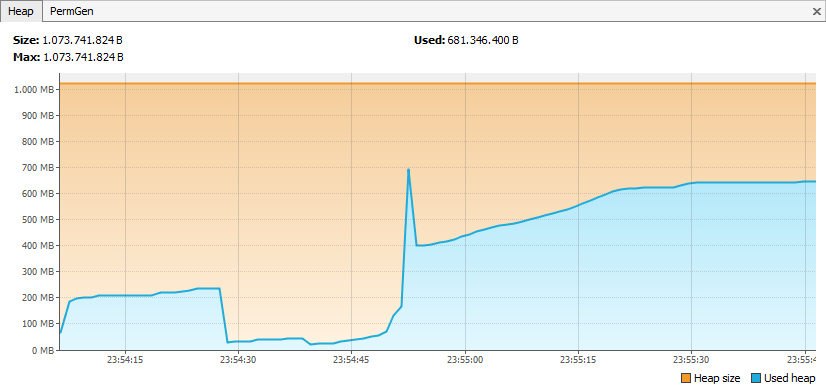
\includegraphics[scale=0.7]{mitFehler.png} \caption{Auswertung der Performance mit Fehler}
\end{figure}

Den Fehler fanden wir in der Ansichtsklasse. Dort wurde die Größe des Tabellenfensters bei jeder Änderung um das Zweifache erhöht. Dies hatte keinerlei Auswirkungen auf die GUI, doch die immer größer werdenden double-Werte sprengten den Rahmen des Heaps, verlangsamten das Programm stark und machten es fast unbenutzbar.\\
Gelöst wurde das Problem, indem die GridHeight des GridBagConstraits der Ansicht bei Diagramm- und Kartenfenster auf 1 und bei Tabellenfenster auf 2 gesetzt wurde. So sieht die Analyse der JVisualVM nach dem beheben des Fehlers aus, wenn man schnell Gebiete wechselt:\\
\begin{figure}[!ht]
\centering
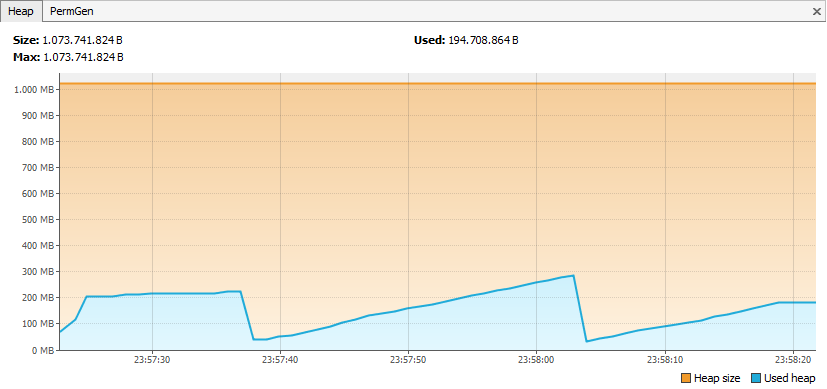
\includegraphics[scale=0.7]{ohneFehler.png} \caption{Auswertung der Performance ohne Fehler}
\end{figure}

\section{Sonstiges}

\subsection{Zusätzliche Features}
\begin{itemize}
\item{\bf{Sortierung}}\\
Ein Feature, wozu wir in der Implementierungsphase nicht gekommen sind, weil es uns zu aufwendig vorkam, ist die Sortierung der Tabellen durch Klicken auf die Köpfe. Dies wurde jetzt realisiert, da es sich als doch nicht so schwer herausstellte. Es wurde ein TableRowSorter im Wahlvergleichs-, Tabellen- und Berichtsfenster eingefügt und konfiguriert.\\

\item{\bf{Debug Klasse}}\\
Während der Validierungsphase hielten wir es für notwendig strukturiert mit Debug Meldungen umzugehen. Aus diesem Grund wurde eine Debug Klasse implementiert, die dazu dient Debug Meldungen aktivieren und deaktivieren zu können. Es können außerdem unterschiedliche Debug Levels verwendet werden um den Überblick zu behalten.

\end{itemize}

\subsection{Änderungen}
\begin{itemize}


\item{\bf{Webview}}\\
Alle Webviews (About, Handbuch, Lizenz) wurden durch JFrames ersetzt, weil es unter Linux zu Komplikationen kam. Jetzt sind die Fenster auch unter Linux lauffähig.\\

\item{\bf{Simulation des negativen Stimmgewichts}}\\
TODO

\item{\bf{Wahlgenerator}}\\
Es gibt nur noch einen Wahlgenerator und es ist somit nicht mehr nötig eine abstrakte Oberklasse für diesen Wahlgenerator zu haben. Diese Oberklasse wurde entfernt.

\item{\bf{Handbuch}}\\
TODO

\item{\bf{Chronik}}\\
TODO

\end{itemize}

\section{Ausblick auf die Endphase des Projekts}


\begingroup
\parindent 0pt
\parskip 2ex
\def\enotesize{\normalsize}

\endgroup
\end{document}
